\section{Natural Language Generation in Antiquity}
 
The desire to build algorithms and machines that generate natural language has
an extensive history in both art and science, as well as spiritual practice,
and especially soothsaying and prognostication.  One early account of a
language generation algorithm comes from 14\textsuperscript{th} century
historian `Abd ar-Rahm\={a}n ibn Khald\={u}n (1332 -- 1406), who writes in his
universal history, the \textit{Muqaddimah} (1377), of a circular
prognostication and divining tool  used by Sufi mystics called a
z\={a}'irjah.\footnote{Franz Rosenthal in his English translation of the
\textit{Muqaddimah} suggests the name is derived from the Persian words
z\={a}'icha meaning ``horoscope'' or  ``astronomical table'' and d\={a}'ira
meaning ``circle.''} Its practice is \begin{quote} ``a branch of the science of
letter magic, practiced among the authorities on letter magic, is the technique
of finding out answers from questions by means of connections existing between
the letters of the expressions used in the question.''\end{quote}

Ibn Khald\={u}n points to an earlier treatise by the Sufi scholar Abu al-Abbas
as-Sabti (1129 -- 1204) of Marrakesh as a source of instructions for the
device's use, suggesting the practice is at least as old at the
12\textsuperscript{th} century \citep{rosenthal1958muqaddimah}.

\begin{figure}
\centering
  
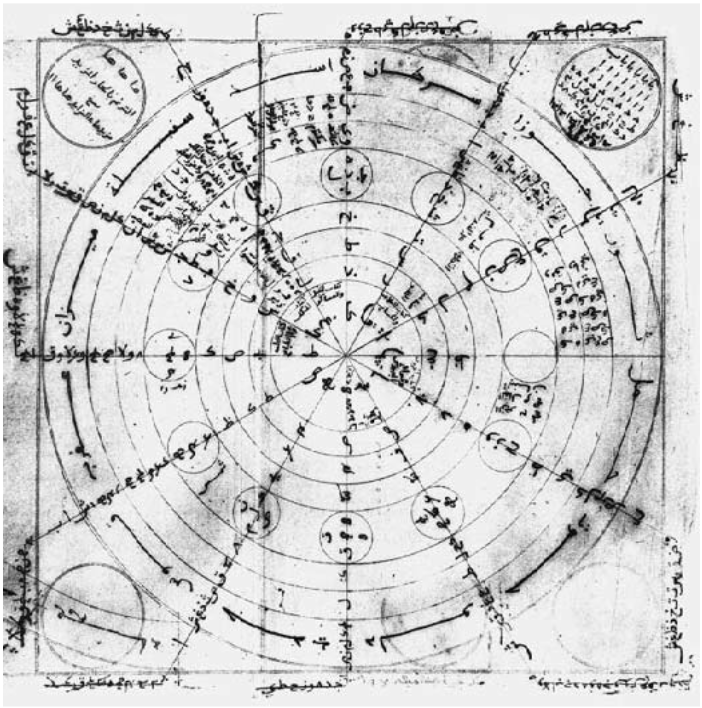
\includegraphics[width=0.49\textwidth]{ch2/images/zairjah_front.png}
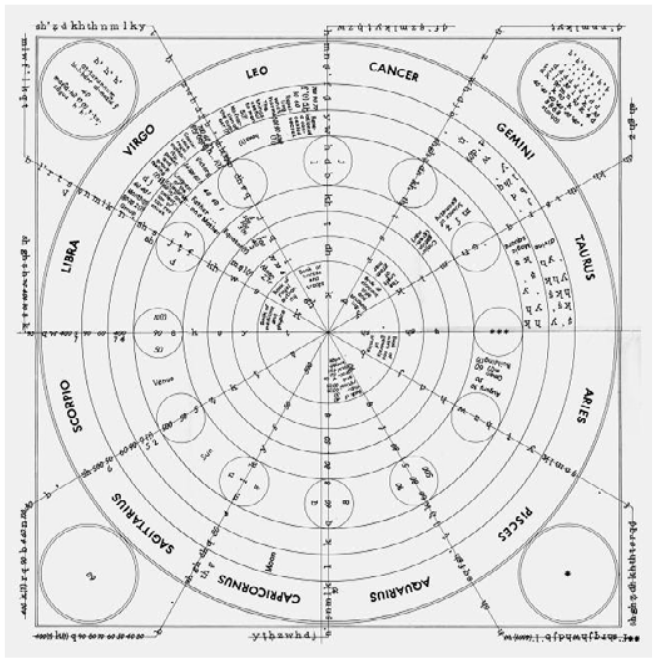
\includegraphics[width=0.49\textwidth]{ch2/images/zairjah_front_translation.png}\\
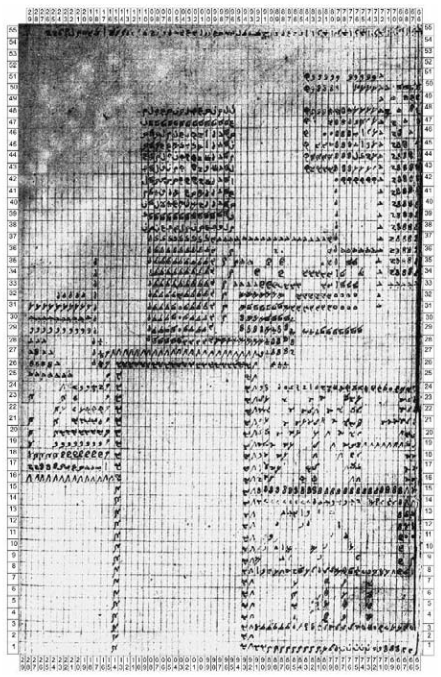
\includegraphics[width=0.6\textwidth,angle=90]{ch2/images/zairjah_back.png}
  
\caption{A z\={a}'irjah from a 15\textsuperscript{th} century Turkish
manuscript of the \textit{Muqaddimah} (top left), its English translation from
\cite{rosenthal1958muqaddimah} (top right), and its lookup table (bottom).
Images taken from \cite{link2010variantology}.}
\label{fig:zairjah}

\end{figure}

 
The z\={a}'irjah itself consists of a series of concentric circles divided into
12 sections by six chords. The various segments of the diagram are annotated
with letters and numerals. Additionally, the z\={a}'irjah is accompanied by a
lookup table mapping letters to numbers. See \autoref{fig:zairjah} for an
example. According to painstaking reconstructions done by
\cite{link2010variantology}, a ``key poem'' was used to pose a question to the
z\={a}'irjah and serve as a mnemonic device/mapping of letters to entries in
the lookup table.  A combination of rules and astronomical observations
(antiquity's equivalent of a random seed) were then applied to the key poem to
read off series of characters from the z\={a}'irjah. The operator would then
interpret those letters into an answer.  ``The fact that only consonants are
written down in Semitic languages permits the meaningful interpretation of many
random permutations of symbols,'' \citep{link2010variantology} suggesting that
cherry-picking outputs and over-ascribing intelligence, knowledge, and even
wisdom, to a language generation algorithm are as old as the practice of NLG
itself.
  
In a secondary account from a manuscript found at the library of Rabat in
Morroco, it is written that a skeptical ibn Khald\={u}n asked of the device how
old it was, ``[Is the] z\={a}'irjah [a] recent or [an] ancient science?''
Allegedly he received the answer, ``The  Holy  Spirit  will  depart,  its
secret having been brought forth / To Idr\={\i}s, and through it, he ascended
the highest summit,'' connecting the practice to the sage Idr\={\i}s who is one
of the eldest ancestors in the Quranic tradition
\citep{rosenthal1958muqaddimah,link2010variantology}.
  
The teachings of Arabic mystics, including the practice of z\={a}'irjah, as
well as the Kabbalistic tradition embodied in the \textit{Sefer Yetzirah} are
known to have strongly influenced the Majorcan Christian mystic, Ramon Llull
(1232-1315) \citep{kahn1980,link2010variantology,sepllull}.  Llull, who is
regarded as an early philosopher of combinatorics, logic, and computation
\citep{bonner2007art,knuth2013art,sepllull}, developed a computational system
based on moveable concentric circles made of paper and connected by string.
The workings of these \textit{volvelle}\footnote{The name \textit{volvelle}
comes from the Latin, literally ``to turn.''} are described in his master work,
\textit{Ars Magna} (1305). According to his system, concepts were assigned
letters which were manipulated to generate new statements involving the
concepts, and  he claimed could be used to determine the truth of any
proposition \citep{Crupi2019VolvellesOK}. Llull's work is also thought to have
influenced the polyalphabetic substitution cipher developed by Leon Battista
Alberti (1404 -- 1472) (see \autoref{fig:llull_volvelle}), the same core
cryptographic technology used in the Enigma machine  \citep{kahn1980}.

\begin{figure}[t]
    \centering

    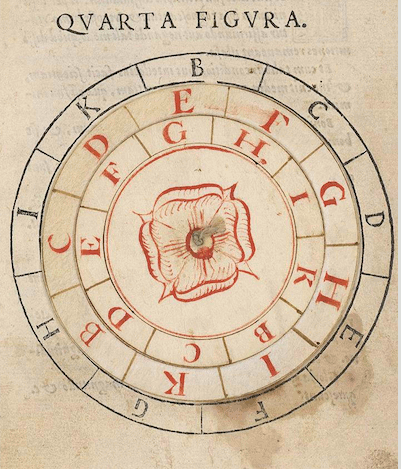
\includegraphics[width=0.45\textwidth]{ch2/images/llull_volvelle.png}\hfill
    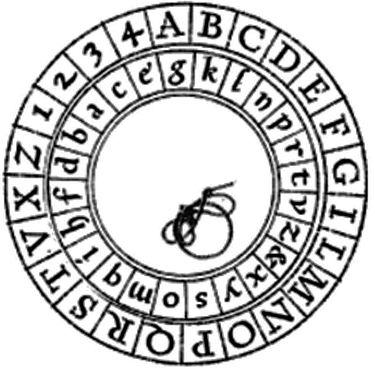
\includegraphics[width=0.45\textwidth]{ch2/images/alberti_cipher_disk.jpg}

\caption{(Left) A volvelle from  Llull's \textit{Ars Magnus} and (right)
Alberti's cipher disk.}
\label{fig:llull_volvelle}
\end{figure}


\begin{figure}[p]
    \centering
    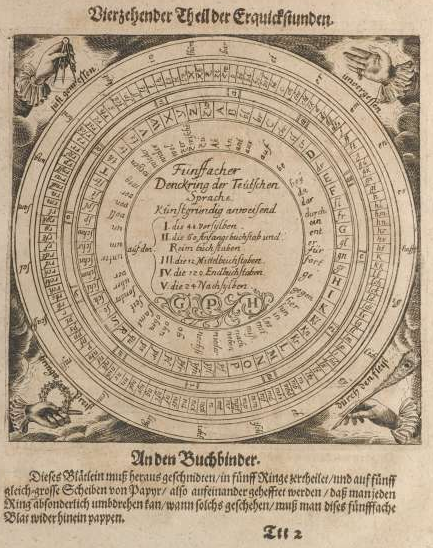
\includegraphics[width=0.98\textwidth]{ch2/images/baroque_volvelle.png}
  
\caption{An illustration of the German word generator volvelle, \textit{F{\"u}nffacher
Denckring der Teutschen Sprache} (1651) by Georg Philipp Harsd{\"o}rffer.}
\label{fig:baroque_volvelle}

\end{figure}
 
 
Llull's use of the volvelle as generative device was influential throughout
medieval Europe, where volvelle were used in both art and science. Arguably
they reached their zenith in the baroque works of Georg Philipp Harsd{\"o}rffer
(1607 -- 1658). His master work volvelle, \textit{F{\"u}nffacher Denckring der
Teutschen Sprache} (1651), consisted of five paper discs (depicted in
\autoref{fig:baroque_volvelle}), and was designed to model German word
formation. It was also advertised as an aid in the production of poems and
other literary  forms \citep{schafer2006literary}.
  
While computational devices before modern computing were limited in complexity
by their construction materials, chiefly paper, the dream of speaking automata
was also alive in myth.  See for example \autoref{fig:brazen_head}, in which a
17\textsuperscript{th} century woodcut print depicts a talking head capable of
answering any question. This ``brazen head'' was allegedly built by the monk
Roger Bacon, who in addition to being an early philosopher of science and
linguist, might also be considered the first NLP engineer if folklore is true
\citep{hyman2016automaton,sep-roger-bacon}.

\begin{figure}
    \centering
    \noindent
    {%
        \setlength{\fboxsep}{0pt}%
        \setlength{\fboxrule}{1pt}%
        \fbox{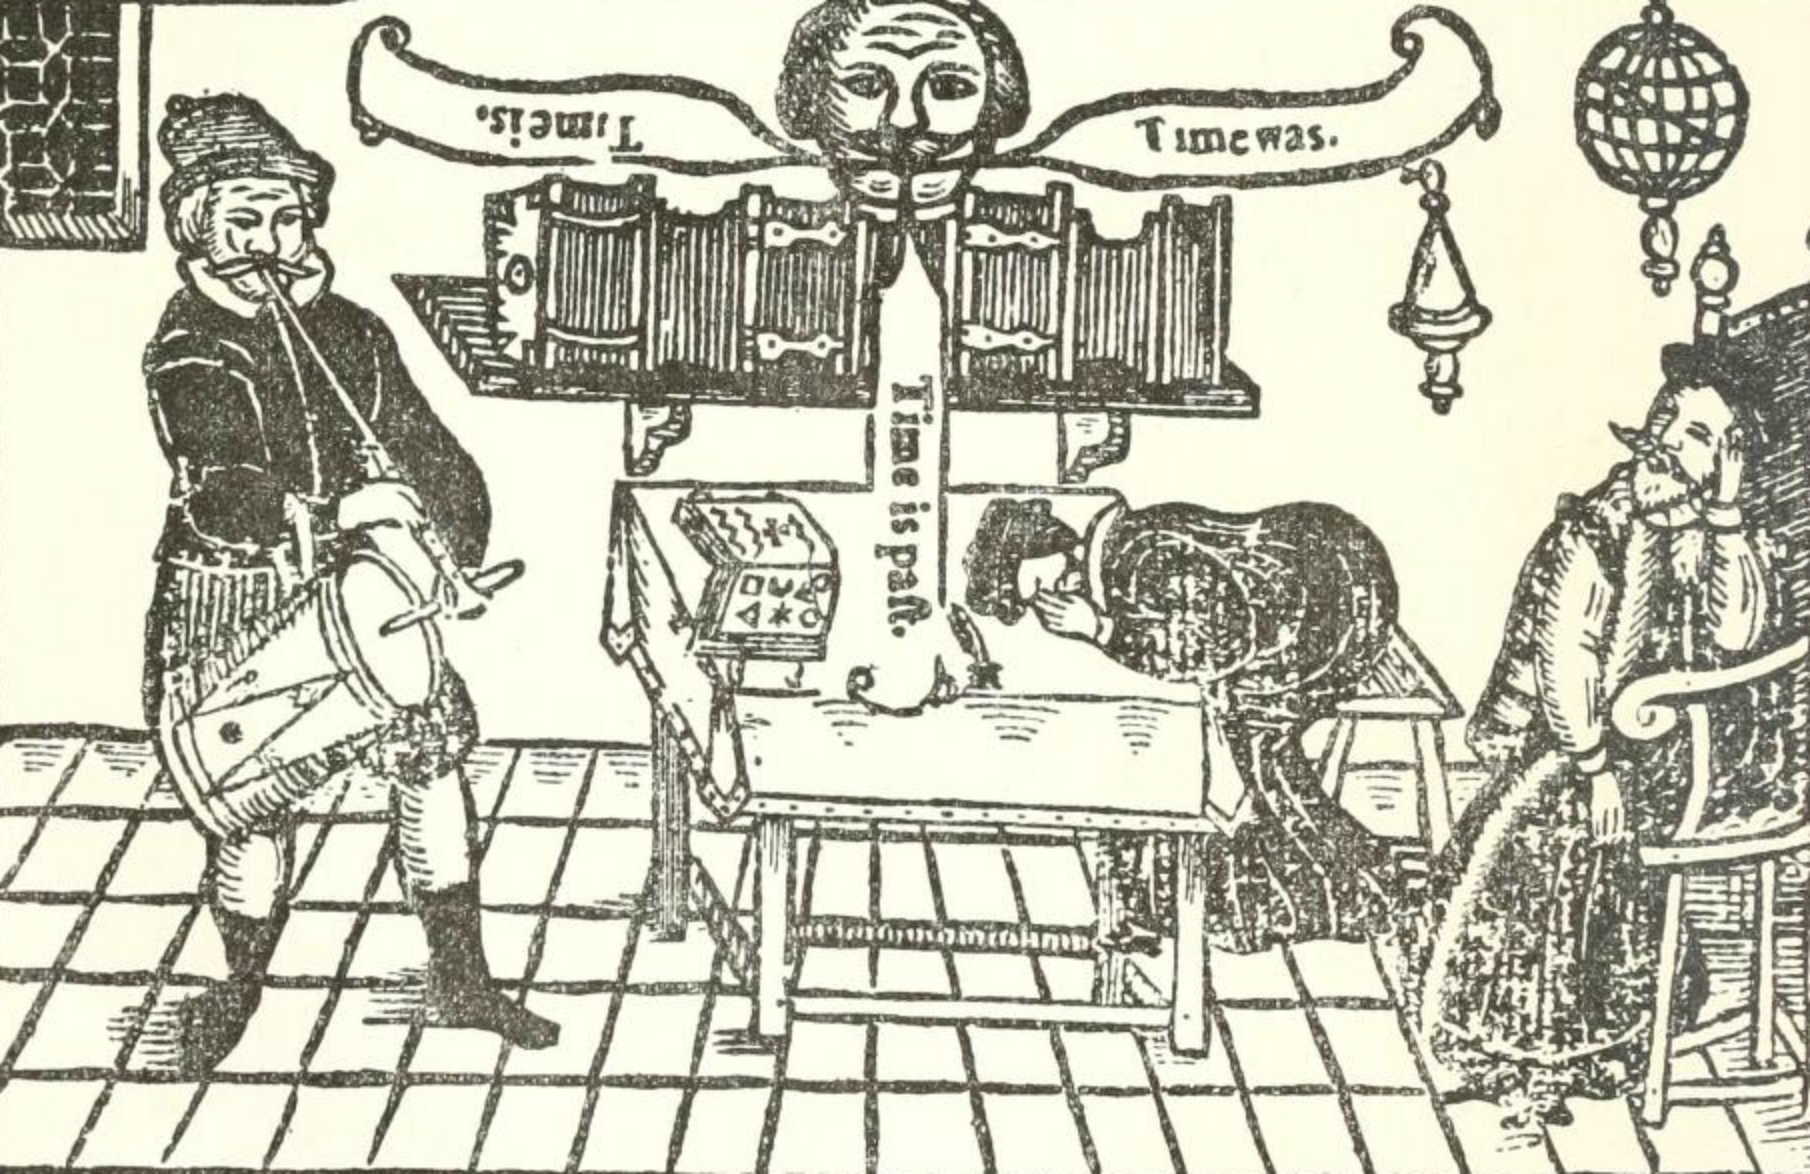
\includegraphics[width=0.7\textwidth]{ch2/images/brazen_head.png}}
    }

\caption{A 1630 woodcut depicting Roger Bacon's talking bronze head, a
mischievious talking autamata allegedly capable of answering any question.
Image taken from \cite{hyman2016automaton}.}
\label{fig:brazen_head}

\end{figure}
 
 
